\documentclass[tikz,border=1cm]{standalone}
\usepackage{newtxmath}
\usetikzlibrary{angles,quotes,spath3}
\everymath{\displaystyle}
\usepackage{amsmath}
\usepackage{fixdif}
\usepackage{derivative}
\tikzset{
    every label/.style={inner sep=0pt,outer sep=0pt},
    notation/.style={-latex,very thick},
    }
\begin{document}
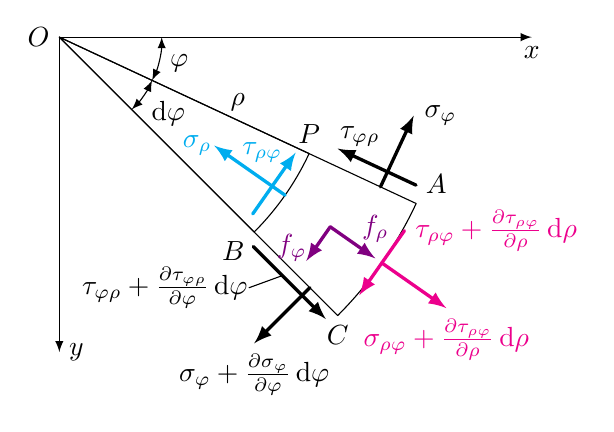
\begin{tikzpicture}[line join=round,line cap=round]
    \draw[-latex] (0,0) -- (6,0) node[label=below:$x$] (X) {};
    \draw[-latex] (0,0) -- (0,-4) node[label=right:$y$] (Y) {};
    \draw (0,0) node[label=left:$O$] (O) {} -- (-25:5) node[label=above right:$A$] (A) {} arc (-25:-45:5) node[label=below:$C$] (C) {} -- cycle;
    \draw (0,0) -- (-25:3.5) node[label=$P$] (P) {} arc (-25:-45:3.5) node[label=below left:$B$] (B) {} -- cycle;
    \pic[draw,latex-latex,angle radius=1.3cm,"$\d\varphi$",angle eccentricity=1.3] {angle = C--O--A};
    \pic[draw,latex-latex,angle radius=1.3cm,"$\varphi$",angle eccentricity=1.2] {angle = A--O--X};
    \draw[notation,magenta] (-35:5) -- (-35:6) node[label=below:$\sigma_{\rho\varphi}+\pdv{\tau_{\rho\varphi}}{\rho}\d\rho$] {};
    \path[spath/save=curve] (A) arc (-25:-45:5);
    \draw[notation,magenta,spath/transform to={curve}{0.5}] (-.5,0) node[right] {$\tau_{\rho\varphi}+\pdv{\tau_{\rho\varphi}}{\rho}\d\rho$} -- (.5,0);
    \draw[notation,violet] (-35:4.2) -- (-35:4.9) node[above=2pt] {$f_\rho$};
    \draw[notation,violet] (-35:4.2) -- ++(-125:.53) node[above left=-4pt] {$f_\varphi$};
    \draw[notation,cyan] (-35:3.5) -- (-35:2.4) node[left=-3pt] {$\sigma_\rho$};
    \draw[notation,cyan] (-35:3.3) ++(-125:.43) -- ++(55:.95) node[left=1pt] {$\tau_{\rho\varphi}$};
    \draw[notation] (-25:4.5) -- ++(65:1) node[right]{$\sigma_\varphi$};
    \draw[notation,shift={(65:6pt)}] (-25:4.9) -- (-25:3.8) node[above right=-3pt] {$\tau_{\varphi\rho}$};
    \draw[notation] (-45:4.5) -- ++(-135:1) node[below]{$\sigma_\varphi+\pdv{\sigma_\varphi}{\varphi}\d\varphi$};
    \draw[notation,shift={(-125:4pt)}] (-45:3.6) -- node[pos=.4] (N) {} (-45:4.9);
    \node[above] at (-25:2.5) {$\rho$};
    \draw (N.base) -- ++(-160:.45) node[left=-3pt] {$\tau_{\varphi\rho}+\pdv{\tau_{\varphi\rho}}{\varphi}\d\varphi$};
\end{tikzpicture}
\end{document}